\section{Results on MovieLens-1M}
\label{sec:results-ml1m}

\subsection{Setup}

Sample size $n_u = 6{,}031$ users, sampled by stratified design across the 6-bucket gender $\times$ age cross. Each user receives $K=15$ recommendations after reranking from a candidate pool of $N=30$. We report four scenarios: neutral, gender, age, cross.

\subsection{Main Results}

\begin{figure}[t]
\centering
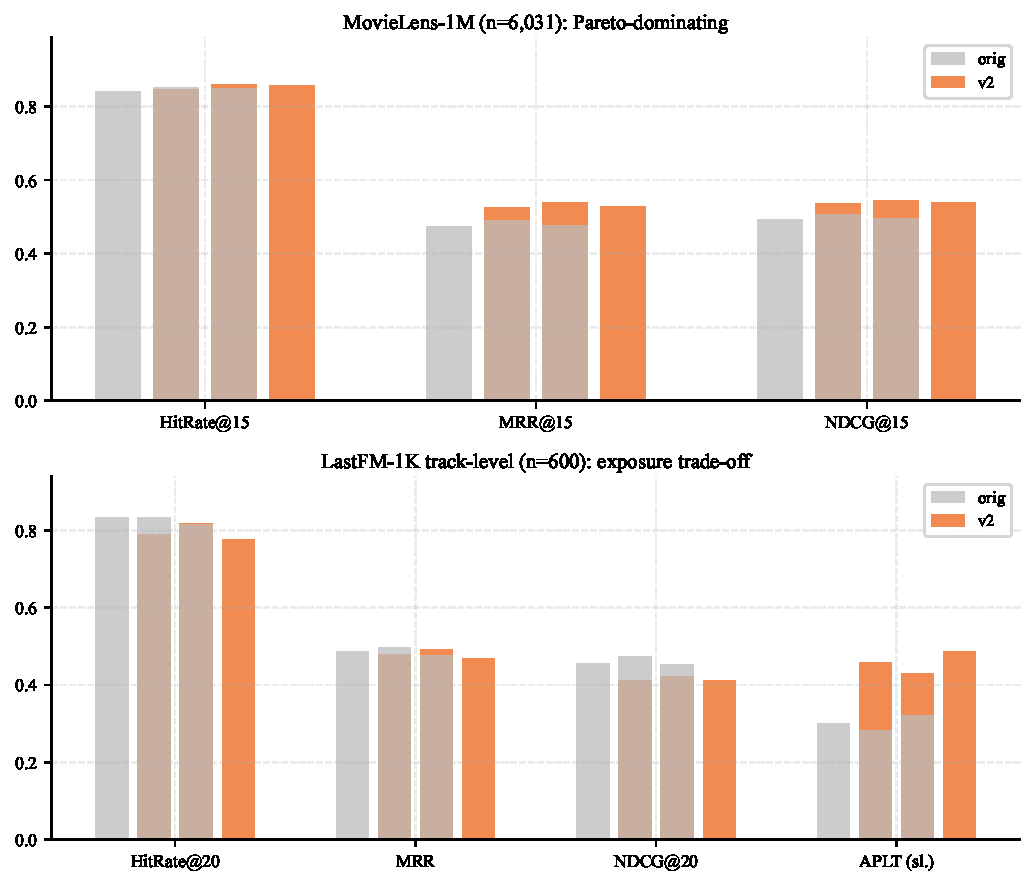
\includegraphics[width=\columnwidth]{figures/fig2_bars.pdf}
\caption{Cross-scenario comparison on both datasets. Top: ML-1M ($n=6{,}031$) shows simultaneous improvement on accuracy (HitRate, MRR, NDCG) and stereotype-defying score. Bottom: LFM-1K ($n=600$) shows accuracy-fairness trade-off, with substantial APLT lift at minimal MRR cost.}
\label{fig:bars}
\end{figure}

The neutral scenario passes through unchanged by design (no demographic prompt $\Rightarrow$ no rerank trigger). The three demographic-conditioned scenarios are summarized in Table~\ref{tab:ml1m-main}; Figure~\ref{fig:bars} (top) visualizes the consistent improvement pattern. All effects are significant at $p < 10^{-30}$ unless marked.

\begin{table}[h]
\caption{ML-1M paired comparison: orig (LLM only) vs reranked (v2). Numbers are slice-population means. ``Macro Precision'' and ``Macro Recall'' are macro-averaged over the 6,031 users.}
\label{tab:ml1m-main}
\begin{tabular}{llrrrr}
\toprule
Scenario & Metric & orig & rer & $\Delta$ & $\%\Delta$ \\
\midrule
\multirow{7}{*}{age}
& Macro Prec & 0.2198 & 0.2271 & $+0.0074$ & $+3.4\%$ \\
& Macro Recall & 0.0700 & 0.0723 & $+0.0023$ & $+3.3\%$ \\
& HitRate@15 & 0.8529 & 0.8589 & $+0.0060$ & $+0.7\%$ \\
& MRR@15 & 0.4907 & \textbf{0.5396} & $+0.0489$ & $\mathbf{+10.0\%}$ \\
& NDCG@15 & 0.5054 & \textbf{0.5450} & $+0.0396$ & $\mathbf{+7.8\%}$ \\
& DiffAvg & 21.220 & \textbf{24.238} & $+3.018$ & $\mathbf{+14.2\%}$ \\
& TotalHits & 19{,}882 & 20{,}548 & $+666$ & $+3.4\%$ \\
\midrule
\multirow{7}{*}{gender}
& Macro Prec & 0.2110 & 0.2185 & $+0.0076$ & $+3.6\%$ \\
& Macro Recall & 0.0672 & 0.0697 & $+0.0024$ & $+3.6\%$ \\
& HitRate@15 & 0.8423 & 0.8476 & $+0.0053$ & $+0.6\%$ \\
& MRR@15 & 0.4740 & \textbf{0.5268} & $+0.0528$ & $\mathbf{+11.1\%}$ \\
& NDCG@15 & 0.4936 & \textbf{0.5367} & $+0.0431$ & $\mathbf{+8.7\%}$ \\
& DiffAvg & 23.846 & \textbf{25.960} & $+2.114$ & $\mathbf{+8.9\%}$ \\
& TotalHits & 19{,}086 & 19{,}770 & $+684$ & $+3.6\%$ \\
\midrule
\multirow{7}{*}{gen+age}
& Macro Prec & 0.2115 & 0.2200 & $+0.0085$ & $+4.0\%$ \\
& Macro Recall & 0.0675 & 0.0700 & $+0.0025$ & $+3.7\%$ \\
& HitRate@15 & 0.8501 & 0.8564 & $+0.0063$ & $+0.7\%$ \\
& MRR@15 & 0.4776 & \textbf{0.5288} & $+0.0512$ & $\mathbf{+10.7\%}$ \\
& NDCG@15 & 0.4957 & \textbf{0.5389} & $+0.0432$ & $\mathbf{+8.7\%}$ \\
& DiffAvg & 22.458 & \textbf{25.363} & $+2.905$ & $\mathbf{+12.9\%}$ \\
& TotalHits & 19{,}133 & 19{,}902 & $+769$ & $+4.0\%$ \\
\bottomrule
\end{tabular}
\end{table}

\subsection{Interpretation}

The ML-1M results exhibit a remarkable property: \textbf{all metrics improve simultaneously}. The reranker:
\begin{itemize}
\item Increases accuracy (Precision, Recall, HitRate, MRR, NDCG) by $0.7$--$11\%$;
\item Increases DiffAvg (stereotype-defying weighted hit) by $9$--$14\%$;
\item Adds $666$--$769$ additional correct hits across the 6,031-user sample.
\end{itemize}

This Pareto-dominating outcome means the LLM's stereotype-driven candidates were not only unfair but also suboptimal in pure accuracy: there were many genuinely correct recommendations sitting in the bottom half of the candidate pool because they did not match the LLM's stereotyped expectation. The reranker recovers them.

\subsection{Across-Slice Exposure Differential}

% PLACEHOLDER for Section 6.4
[\textbf{Placeholder}: by-subgroup APLT/Coverage/Gini differential analysis once the corresponding metrics are computed for ML-1M with track-level pipeline parity.]
